\section{Benutzeroberfläche}
\subsection{Hauptbildschirm}

\begin{figure}[H]
    \centering
    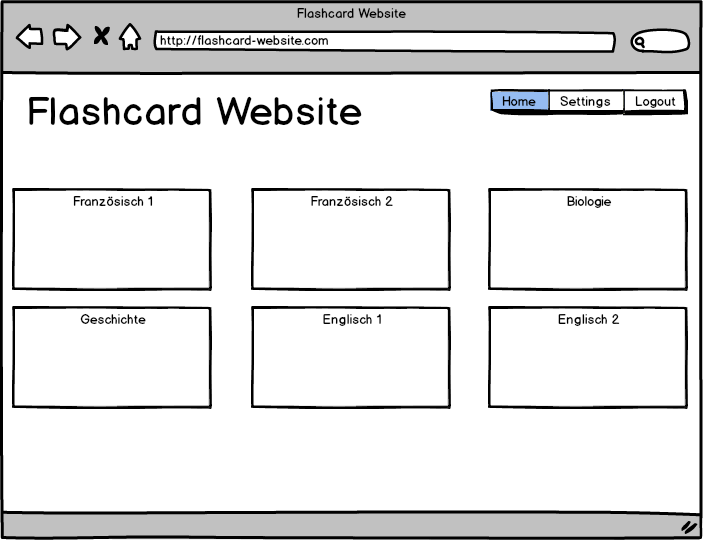
\includegraphics[width=0.7\textwidth]{images/Overview.png}
    \caption{Hauptbildschirm}
    \label{fig:overview}
\end{figure}

Der Hauptbildschirm gibt eine Übersicht zu den Karteikartensets des angemeldeten Benutzers. Beim Klicken auf eines der Sets kommt man zum Lernbildschirm


\subsection{Lernbildschirm}


\begin{figure}[H]
    \centering
    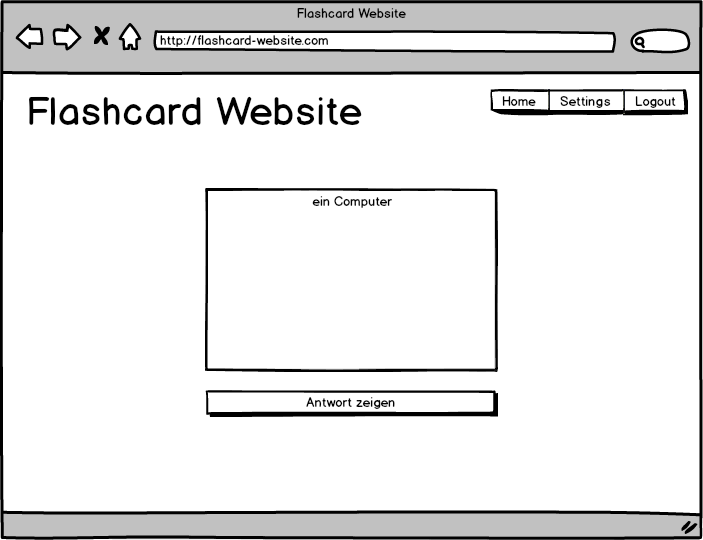
\includegraphics[width=0.7\textwidth]{images/Lernscreen-Frage.png}
    \caption{Frageseite einer Karteikarte}
    \label{fig:lernscreen-frage}
\end{figure}

\begin{figure}[H]
    \centering
    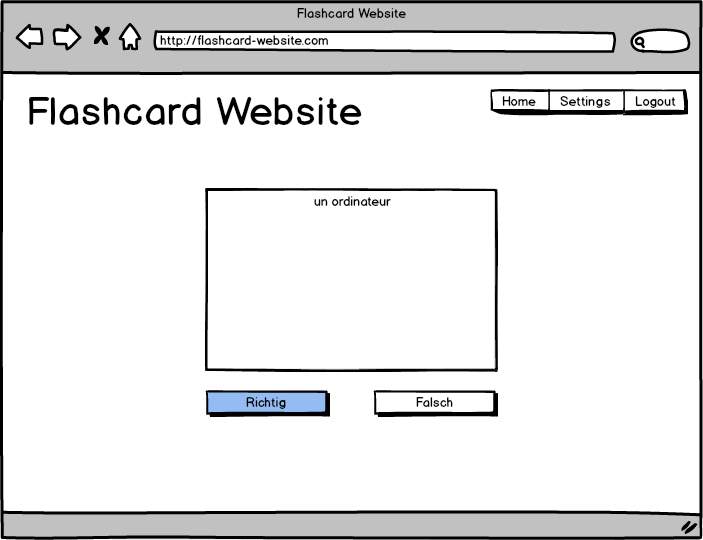
\includegraphics[width=0.7\textwidth]{images/Lernscreen-Antwort.png}
    \caption{Antwortseite einer Karteikarte}
    \label{fig:lernscreen-antwort}
\end{figure}

Der Lernbildschirm fängt mit der Vorderseite von der ersten Karteikarte des Sets an. Wenn man sich die Rückseite mit der Antwort anzeigen lässt, hat man die Möglichkeit anzugeben, ob man richtig lag oder nicht.

\begin{figure}[H]
    \centering
    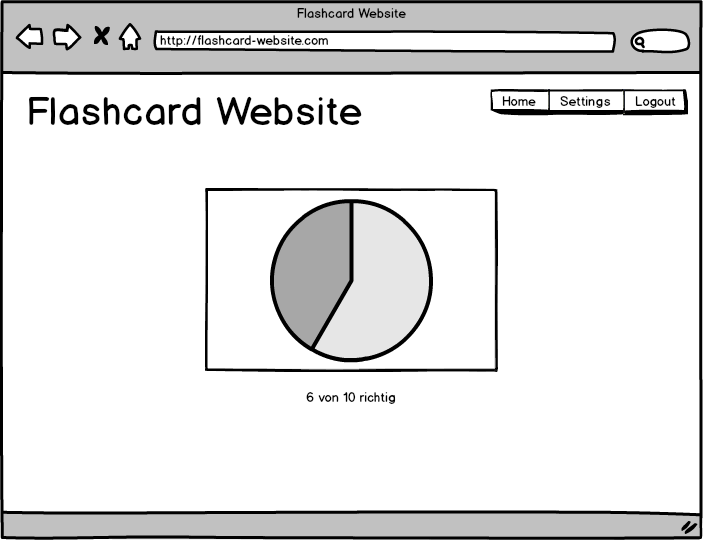
\includegraphics[width=0.78\textwidth]{images/Lernscreen-Ergebnis.png}
    \caption{Ende des Karteikartensets}
    \label{fig:lernscreen-ergbenis}
\end{figure}

Nachdem man alle Karteikarten durchgegangen ist, wird eine Statistik zu der Anzahl an richtigen Antworten angezeigt.
